\section{Роль дифракции в приборах, формирующих изображение. Критерий Рэлея (применительно к формированию изображений). Дифракционный предел разрешения телескопа и микроскопа.}

Из-за наличия во Вселенной дифракции Фраунгофера на круглом отверстии, вместо точки при фокусировке света мы получаем небольшое пятнышко, которое называется \textbf{пятном (диском) Эйри}. Его радиус можно рассчитать по следующей формуле:

\begin{equation*}
	\rho_{a} = 1.22 \frac{\lambda}{D} F	
\end{equation*}

Здесь $\lambda$ --- длина волны наблюдаемого излучения, $D$ --- диаметр линзы, $F$ --- ее фокусное расстояние.

Пусть мы наблюдаем некоторый объект, который находится на главной оптической оси. Тогда и его изображение будет находиться там же. Пусть теперь у нас добавляется еще один объект, который находится от первоначального на некотором (небольшом) угловом расстоянии $\psi$. Пятно Эйри от этого объекта в таком случае будет находиться на таком же угловом расстоянии от исходного пятна, а линейное расстояние тогда будет равно $l = F \psi$. 

Для того, чтобы понять, возможно ли эти два объекта разрешить, был введен так называемый \textbf{критерий Рэлея}, который говорит, что минимальное расстояние между объектами, на котором их можно разрешить, оказывается таким, что первый минимум пятна Эйри от одного объекта приходится на нулевой максимум пятна Эйри другого.

С учетом имеющейся у нас формулы для радиуса пятна Эйри мы получим:

\begin{equation*}
	\psi_{min} F = 1.22 \frac{\lambda}{D} F \qrq \boxed{\psi_{min} = 1.22 \frac{\lambda}{D}}
\end{equation*}

Рассмотрим теперь микроскоп. Предположим, что предмет у нас лежит в какой-то среде с показателем преломления $n$ (так делается, например, в диффузионных микроскопах); по другую сторону линзы у нас, соответственно, воздух, с показателем преломления $n_{air} = 1$. Как уже было сказано ранее, от каждой точки предмета будет получаться не точечное изображение, а пятно Эйри. Введем углы $u_1$ и $u_2$ (см. рисунок). Угол $u_1$ называется апертурным углом объектива.

\begin{figure}[H]
	\centering
	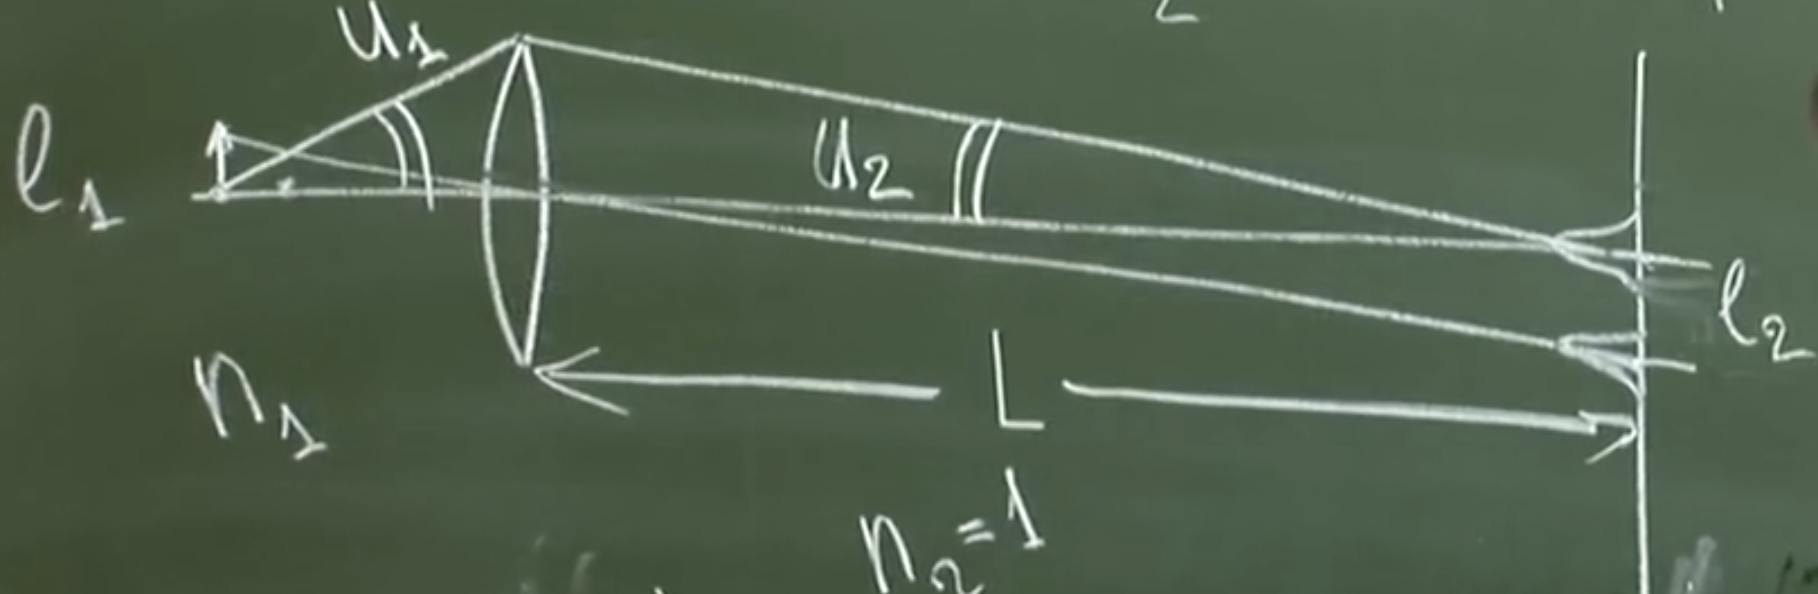
\includegraphics[width=\linewidth]{36_1}
\end{figure}

Как видно из рисунка, верно следующее:

\begin{equation*}
	\frac{D}{L} \approx 2 u_2 \approx 2 \sin u_2
\end{equation*}

Согласно Аббе, идеальный с точки зрения геометрии микроскоп подчиняется следующему условию (\textbf{условие синусов Аббе}):

\begin{equation*}
	l_1 n_1 \sin u_1 = l_2 n_2 \sin u_2 \qrq l_1 n \sin u_1 = l_2 \frac{D}{2L}
\end{equation*}

Здесь $l_1$ и $l_2$ есть линейные размеры предмета и изображения соответственно.

Ну и с учетом критерия Рэлея, который в данном случае удобно сформулировать как "линейный размер изображения должен получаться не меньше радиуса пятна Эйри", мы получим:

\begin{equation*}
	l_{2 min} = \rho_a = l_{1 min} \frac{2 L n\sin u_1}{D} = 1.22 \frac{\lambda}{D} L \qrq l_{1 min} = 0.61 \frac{\lambda}{n\sin u_1}
\end{equation*}

Выражение $n \sin u_1$ в знаменателе называют \textbf{числовой апертурой микроскопа}.